\chapter{Software Architecture}

\epigraphhead{\epigraph{As a rule, software systems do not work well until they
have been used, and have failed repeatedly, in real applications.}{\textit{David Parnas}}}


\section{Data Management}

Data from the \hisparc experiment is stored centrally at Nikhef. The following
requirements have been defined for the \hisparc project:
\begin{enumerate}
    \item need for a well-documented and standardized format
    \item access to the \emph{complete} dataset for all schools
    \item high-bandwidth connection
    \item data integrity
\end{enumerate}
The first requirement is taken care of by publishing the format.  The second
means that there is a central location where either the data itself is stored,
or metadata is stored which describes where to find the data.  The \hisparc
experiment has chosen to store the data in one location. The third requirement
depends on the size of a typical dataset.  For large datasets, to satisfy
the third requirement multiple copies of the data may exist.  In such
cases, (partial) copies are located as close to the researcher as
possible, at a location with high-bandwidth access.\footnote{Including, but
not limited to, the desktop or laptop of the researcher.}  Methods for
data access have been implemented to enable downloading of all the data.
The fourth requirement is solved by backups, as well as strict integrity
checks.  Note that backups and integrity checks should be designed to
prevent both \emph{data loss}, as well as \emph{duplicate} or
\emph{corrupt} data.

Storage may be divided into storage \emph{tiers}.  Storage tiers are different
kind of storage which differ in at least one of four attributes: price,
performance, capacity or function.  For example, the bulk of the data might be
stored on magnetic tape (cheap, but slow), while an array of solid state drives
(fast, but expensive) contain only data currently being analyzed.  The most
expensive storage is usually called \emph{tier 1}, as this contains the most
critical, or recently accessed data.  Lower tiers are usually cheaper, slower,
but with more capacity. Three storage tiers have been implemented for \hisparc.
Tier 1 and 2 will be discussed shortly. Tier 3 is a backup storage on magnetic
tape in a different geographical location from tier 1 and 2.

Data may also be divided into levels.  Loosely following the definition used by
NASA \cite[5]{NASA:1986}, level~0 data is unprocessed, raw data.  Level~1 data
have undergone some form of processing.  Data are supplemented with data like
timestamps and instrument configuration.  Simple processing steps which are
certain not to change during the lifetime of the experiment may be performed.
For example, compressed data may be decompressed and maximum signal heights (in
raw units) may be recorded.  In contrast, conversion of raw units to physical
units is not performed, as detector calibration usually is a complex process
which is likely to be done differently when the project matures.  Level~2 (and
higher level) data \emph{is} converted to physical units, and may thus be
subject to change.

The \hisparc experiment consists of close to a hundred different stations in
several countries, the majority of which are operated by high school teachers
and support staff.  The quality of internet connections varies from school to
school, and connectivity depends on firewalls, proxy servers and anti-virus
software, which are all implemented by the high schools at their own
discretion.  The data management requirements discussed previously, are much
harder to satisfy as long as data remains at the station locations.  It was
decided to implement a system where data is offloaded from the station locations
as quickly as possible and is stored in a central location, where it is easily
accessed.


\subsection{Data Flow}

``Any system should be as simple as possible, but no simpler'' is a variation on
a quote ascribed to Einstein \cite{Einstein:simple}, and relevant to the design
of this system.  The central data storage designed for \hisparc is
called the \emph{datastore}.  The use of a central location ensures that most of
the data management requirements need to be addressed only once.

\figref{fig:dfd-contextlevel} shows a \emph{context-level} data flow diagram
(DFD) for the \hisparc experiment.  Context-level diagrams only show the
interaction between the system under consideration and all external agents,
which act as data sources or data sinks.  In this view, stations act as data
sources which offload event data to the datastore, as quickly as possible.
Teachers, students and researchers working on \hisparc data, denoted as
\emph{users} in the diagram, act as both data sinks (they retrieve data for
analysis) and data sources (results from their analysis may be stored
centrally).

\begin{figure}
\centering
\begin{tikzpicture}
[font=\sffamily,
 every matrix/.style={ampersand replacement=\&,column sep=2cm,row sep=0.2cm},
 source/.style={draw,thick,rounded corners,fill=yellow!20,inner sep=.3cm},
 process/.style={draw,thick,circle,fill=blue!20},
 sink/.style={source,fill=green!20},
 dots/.style={gray,scale=2},
 to/.style={->,>=stealth',shorten >=1pt,semithick,font=\sffamily\footnotesize},
]
\matrix{
\node[source] (station1) {station}; \& \& \node[sink] (user1) {user}; \\
\node[dots] {\vdots}; \& \node[process] (datastore) {datastore}; \& \node[dots] {\vdots}; \\
\node[source] (station2) {station}; \& \& \node[sink] (user2) {user}; \\
};

\draw[to] (station1) -- (datastore) node[midway,above,sloped] {events};
\draw[to] (station2) -- (datastore) node[midway,above,sloped] {events};
\draw[to] (datastore) to[bend left=10] node[midway,above,sloped] {datasets} (user1);
\draw[to] (user1) to[bend left=10] node[midway,below,sloped] {results} (datastore);
\draw[to] (datastore) to[bend left=10] node[midway,above,sloped] {datasets} (user2);
\draw[to] (user2) to[bend left=10] node[midway,below,sloped] {results} (datastore);
\end{tikzpicture}

\caption{\captitle{Context-level data flow diagram (DFD) of \hisparc.}
Stations pass events to the datastore, where they are accessible to users.
Apart from raw event data, histogrammed data and selected datasets are
also made available.  Using special tools, users can even submit some
results from analysis.}
\label{fig:dfd-contextlevel}
\end{figure}

Of course, this is a very simplistic view.  It does not specify how stations
internally handle data, or which processes handle user requests.  Context-level
DFDs are exploded in a level~0~DFD, or \emph{system-level}~DFD, shown in
\figref{fig:dfd-level0}. The system is divided into processes and data stores.
How the processes work internally is not yet shown.  The
\emph{station PC} process is running on PCs connected to the detector
hardware.
For every station, there is such a process.  The other processes are
unique.
There exist only single copies, and they all run on servers located at Nikhef,
Amsterdam.  We've strived to strike a balance between maintainability (do as
much work as possible on the server, to which we have easy access), and
performance (do work on the station PCs, of which there are many).  The result
is that raw data (level~0) is processed on the station PCs and the resulting
level~1 data is sent to the datastore writer process.  No further
processing of the data itself is required before storage.

There are only two more processes accessing the datastore.  The \hisparc
quicklook generator generates daily histograms from event data and stores them
in the public database.  These quicklooks can be accessed on the web, at
\url{http://data.hisparc.nl/}.  This website is served by the public database
access process.  This process also serves level~1 event data to
users for detailed analysis. The results from the analysis are stored in the
public database.

\begin{figure}
\centering
\begin{tikzpicture}
[font=\sffamily,
 node distance=3cm and 4.5cm,
 source/.style={draw,thick,rounded corners,fill=yellow!20,inner sep=.3cm},
 process/.style={draw,thick,circle,fill=blue!20},
 sink/.style={source,fill=green!20},
 datastore/.style={draw,very thick,shape=datastore,inner sep=.3cm},
 dots/.style={gray,scale=2},
 to/.style={->,>=stealth',shorten >=1pt,semithick,font=\sffamily\footnotesize},
 every node/.style={on grid,align=center},
]

\node[source] (station) {station};
\node[process,below=of station] (stationpc) {station\\pc};
\node[process,right=of stationpc] (writer) {datastore\\writer};
\node[datastore,below right=3cm and 3cm of writer] (datastore) {datastore};
\node[process,below left=3cm and 3cm of datastore] (access) {public\\access};
\node[process,below right=3cm and 3cm of datastore] (quicklook) {quicklook\\generator};
\node[datastore,below=6cm of datastore] (publicdb) {publicdb};
\node[sink,left=of access] (users) {users};

\draw[to] (station) -- (stationpc) node[midway,right] {raw events\\level 0};
\draw[to] (stationpc) -- (writer) node[midway,above] {events} node[midway,below] {level 1};
\draw[to] (writer) to[out=0,in=90] node[near start,above,sloped] {events} node[near start,below,sloped] {level 1} (datastore);

\draw[to] (datastore) to[out=-80,in=90] node[midway,above] {events} node[midway,below] {level 1} (quicklook);
\draw[to] (datastore) to[out=-100,in=90] node[midway,above] {events} node[midway,below] {level 1} (access);

\draw[to] (quicklook) to[out=-90,in=90] node[midway,above] {histograms\\coincidences} node[midway,below] {level 2} (publicdb);

\draw[to] (access) to[out=0,in=100] node[near start,above,sloped] {results} node[near start,below,sloped] {level 3} (publicdb);
\draw[to] (publicdb) to[out=110,in=-90,looseness=1.3] node[midway,above] {histograms\\coincidences} node[midway,below] {level 2} (access);

\draw[to] (access) to[bend left] node[midway,above] {histograms\\coincidences\\events} node[midway,below] {level 1, 2} (users);
\draw[to] (users) to[bend left] node[midway,above] {results} node[midway,below] {level 3} (access);

\node[draw,dashed,very thick,black!60,fit=(writer) (datastore) (access) (quicklook) (publicdb),inner sep=.3cm] (domain) {};
\node[black!60,below=10pt of domain.north] {\textbf{\Large Nikhef}};
\end{tikzpicture}

\caption{\captitle{Level~0 data flow diagram.}  This diagram shows some
more detail.  Each station has a dedicated PC running the data acquisition
software.  Event data are sanitized and some preliminary analysis results and
configuration settings are added.  The results are then sent to the datastore.
The process handling public data access reads events from the datastore and
stores selected events and histogrammed data in the public database.  Users can
then access this data.}
\label{fig:dfd-level0}
\end{figure}


\subsection{Station PC}

Every \hisparc station is equipped with a dedicated PC controlling and
reading out the detectors.  The PC is connected to the \hisparc
electronics.  The dataflow of a station PC is shown in
\figref{fig:dfd-stationpc}.  The \daq process communicates with the
electronics unit. In the case of a master / slave combination, two raw
event messages (one for each device) make up an event and three GPS
one-second messages\footnote{Once a second, the GPS module sends out a
data message containing the current time and several data values needed
for correcting quantization errors.  In total, three one-second messages
are needed to obtain all the necessary values for correcting the
timestamp of a particular event.} are needed to calculate an accurate GPS
timestamp for the event.  The event data is analyzed and baseline,
pulseheights and integrals are calculated and added to the event messages.
These events are then stored on disk in the \emph{buffer}, a MySQL
database. The \emph{monitor} process reads data from the buffer.  The
event messages are unpacked and cast in a format which can be easily
parsed by the datastore processes.  After processing, these events are
stored on disk, in the \emph{storage}, an SQLite database.  When a certain
number of events are stored\footnote{User-configurable, but the default
value is 100 events} the data is uploaded to the datastore.  If the
datastore is temporarily unavailable, e.g.  due to the loss of an internet
connection at the school, the storage is designed to hold a substantial
backlog. Once the datastore is available again the backlog is uploaded in
batches.\footnote{Again user-configurable, but the default maximum batch
size is 1000 events}

\begin{figure}
\centering
\begin{tikzpicture}
[font=\sffamily,
 every matrix/.style={ampersand replacement=\&,column sep=2cm,row sep=2cm},
 source/.style={draw,thick,rounded corners,fill=yellow!20,inner sep=.3cm},
 process/.style={draw,thick,circle,fill=blue!20},
 sink/.style={source,fill=green!20},
 datastore/.style={draw,very thick,shape=datastore,inner sep=.3cm},
 dots/.style={gray,scale=2},
 to/.style={->,>=stealth',shorten >=1pt,semithick,font=\sffamily\footnotesize},
 every node/.style={align=center},
]
\matrix{
\node[source] (hisparcbox) {electronics}; \& \node[process] (daq) {DAQ};
\&
\\
\& \node[datastore] (buffer) {buffer}; \& \\
\node[datastore] (storage) {storage}; \& \node[process] (monitor) {monitor}; \& \node[sink] (datastore) {datastore}; \\
};

\draw[to] (hisparcbox) -- node[midway,above] {raw events} node[midway,below] {level 0} (daq);
\draw[to] (daq) -- node[midway,right] {raw event data\\level 1} (buffer);
\draw[to] (buffer) -- node[midway,right] {raw event data\\level 1} (monitor);
\draw[to] (monitor) to[bend right=50] node[midway,above] {events} node[midway,below] {level 1} (storage);
\draw[to] (storage) to[bend right=50] node[midway,above] {events} node[midway,below] {level 1} (monitor);
\draw[to] (monitor) -- node[midway,above] {events} node[midway,below] {level 1} (datastore);
\end{tikzpicture}

\caption{\captitle{Data flow diagram of a \hisparc station PC.}  A \labview
program communicates with the \hisparc II electronics.  Data is
sanitized and, along with preliminary analysis results and configuration
settings, sent to the \emph{buffer}.  The monitor program retrieves raw event
data from the buffer and creates structured array data.  The events are then stored in
the \emph{storage}.  When a batch of events is ready, it is retrieved from
the storage and uploaded over the internet to the datastore.}
\label{fig:dfd-stationpc}
\end{figure}


\subsection{Tier 1: Datastore}

The datastore is the central data storage created for \hisparc. It
receives data from all stations and provides data to all users.  The datastore
is designed to be simple, and efficient.

Stations upload data using HTTP POST requests to the datastore server.  Several
worker processes handle the request.  First, the data's origin is verified by
checking the station number and password.  If the combination is correct, a
checksum is calculated for the payload and compared to the checksum sent in a
POST variable.  If the checksum is verified, the flat data stream is converted
to a data structure.
If that succeeded, the data is assumed to be correct and written to a file in the
\verb|incoming| directory in the datastore's file system.  Finally, a return code
is sent back to the station.  In the event of an error, an error code is
returned.

A single writer process is monitoring the \verb|incoming| directory.  The use of
a single process removes the need for locking or concurrent write access.
Several conventional approaches to locking have proven to be unreliable on
networked filesystems. The writer process opens each file sequentially and the
payload is processed.
The payload is a list of events with a header.  The process writes the event
list to disk in binary files.  Data from all stations is aggregated into single
files for each day.  To keep the number of files per directory small, in the
top-level directory there is a subdirectory for each year, containing
subdirectories for each month.  In these directories are the binary files.  See
\figref{fig:datastore-dir-structure}.

\begin{SCfigure}[50]
\begin{minipage}{.45\linewidth}
\centering
\begin{minipage}{125pt}
\begin{verbatim}
2004/
2005/
...
2011/
    1/
    2/
    ...
    12/
        2011_12_1.h5
        2011_12_2.h5
        ...
        2011_12_31.h5
incoming/
    tmp048r_J
    tmpF7b3se
    tmpj22L8s
    tmpnVBoSh
    tmpZdlj_H
partial/
    tmpFG3c0C
tmp/
    tmpuE0EAM
\end{verbatim}
\end{minipage}
\end{minipage}
\caption{\captitle{Directory structure of the datastore.}  The datastore
contains directories for each year.  Each year contains directories for each
month.  Finally, each month directory contains individual data files.  The name
of each file is simply the date with an extension.  The datastore also contains
directories for temporary files.  The HTTPD daemon writes data files in the
\texttt{tmp/} directory and moves them to the \texttt{incoming/} directory when
finished.  The \texttt{incoming} directory is watched by the datastore writer
process and each file is converted and stored in the final binary data files in
the year/month directories.  During conversion, the writer process keeps the
file in the \texttt{partial/} directory.}
\label{fig:datastore-dir-structure}
\end{SCfigure}

Binary files have several benefits: they are compact (each day's worth of data
is just \emph{one file}, instead of several files in some directory structure,
which is typical for databases), they can easily be backed up (the files do not
change once all data for a single day is received), and they scale linearly.  Of
course, there are also downsides.  Most importantly, the inability to use a
single query\footnote{An SQL query on a relational database, for example.} to,
for example, retrieve several days' worth of data from all stations in a single
cluster.  The downsides are easily mitigated by providing the users with a
higher-level abstraction of the datastore.

The binary files are stored in the open \emph{Hierarchical Data Format, Version
5 (HDF5)} format. This data model is widely used by research organizations and
academia, and is primarily intended for very large and complex datasets.  The
format is also extremely portable\footnote{The HDF5 libraries are available for
almost any computing platform and bindings exist for many languages, including
C, C++, Java and Python.} and can hold data types ranging from simple arrays to
complex gridded data and even pictures. It scales very well from individual
analysis results to data for an entire array of stations.

A higher-level library, \emph{PyTables} \cite{PyTables}, is used to access the
HDF5 files, both for reading and writing.

The structure of an HDF5 file is shown in \figref{fig:datastore-file-structure}.
 The top level \hisparc group contains \emph{groups} for each cluster.  Each
cluster contains groups for each station.  And each station contains several
\emph{tables}: \verb|events| (\hisparc events), \verb|errors| (detector software
error messages), \verb|configs| (detector configuration settings, like
photomultiplier voltage and thresholds), \verb|weather| (optional: weather
station data) and \verb|blobs| (binary, variable length data, like raw event
traces).
\begin{SCfigure}[50]
\begin{minipage}{.45\linewidth}
\centering
\begin{minipage}{160pt}
\begin{verbatim}
hisparc/
    cluster_aarhus/
        station_20002/
        station_20003/
    cluster_amsterdam/
        station_2/
        station_3/
        ...
        station_501/
            blobs
            configs
            events
            errors
            weather
        station_502/
        ...
    cluster_eindhoven/
        station_8001/
        ...
        station_8101/
        ...
    cluster_enschede/
    cluster_groningen/
    cluster_leiden/
    cluster_nijmegen/
    cluster_utrecht/
\end{verbatim}
\end{minipage}
\end{minipage}
\caption{\captitle{File structure of a datastore file.}  A data file first
contains a \texttt{hisparc} group.  In that group, all clusters are represented
by their own group, named after their location.  In each cluster group, there is
a group for each station, named after their \emph{number}, not their location.
Inside a station group are \emph{tables}, containing the actual data.  The
\texttt{blobs} table contains (compressed) binary data from \hisparc events, or
error messages.  The \texttt{events} table contains event data, \texttt{errors}
contains error logs and \texttt{weather} contains data from weather stations
located at \hisparc stations.}
\label{fig:datastore-file-structure}
\end{SCfigure}

The \verb|events| table structure is shown in \tabref{tab:hdf5-events}.  Each
event has a unique\footnote{Unique in this table.  When data is downloaded for
analysis and combined with other data into one table, the \texttt{event\_id}
will be different.  To uniquely define an event, use a station number /
\texttt{ext\_timestamp} combination.} identifier, \verb|event_id|.  Each event
has a Unix timestamp in GPS time, \emph{not} UTC.  The sub-second part of the
timestamp is given in \verb|nanoseconds|.  The \verb|ext_timestamp| is the full
timestamp in \si{\nano\second}.  Since there cannot exist another event with the
same timestamp, this field in combination with the station number uniquely
identifies the event.  The \verb|data_reduction| flag signifies whether the full
PMT trace (\emph{no} reduction) has been stored, or just the PMT pulse
(\emph{reduced}, or \emph{zero suppression}).  The \verb|trigger_pattern| is a
binary value containing the exact trigger condition at the time of the event.
The \verb|baseline|, \verb|std_dev|, \verb|n_peaks|, \verb|pulseheights| and
\verb|integrals| fields are values derived from the PMT traces.  Each field
contains four values, one for each detector.  If a station only has two
detectors, the last two values for each field are \num{-1}.  If the baseline
cannot be determined, all these values are \num{-999}.  The \verb|event_rate| is
the trigger rate at the time of the event.
\begin{table}
\centering
\begin{tabular}{@{}llp{5cm}@{}}
\toprule
Field & Type & Description \\
\midrule
\verb|event_id| & unsigned 32-bit integer & Unique number \\
\verb|timestamp| & 32-bit timestamp & Unix timestamp (GPS) [\si{\second}] \\
\verb|nanoseconds| & unsigned 32-bit integer & Sub-second part of timestamp \\
\verb|ext_timestamp| & unsigned 64-bit integer & Full timestamp (GPS)
    [\si{\nano\second}] \\
\verb|data_reduction| & boolean & Are traces reduced? \\
\verb|trigger_pattern| & unsigned 32-bit integer & Hardware trigger condition\\
\verb|baseline| & signed 16-bit integer (4x) & Baseline of traces [\si{\adc}] \\
\verb|std_dev| & signed 16-bit integer (4x) & Standard deviation of the baseline
    [\si{\adc}] \\
\verb|n_peaks| & signed 16-bit integer (4x) & Number of peaks in data \\
\verb|pulseheights| & signed 16-bit integer (4x) & Pulse height [\si{\adc}] \\
\verb|integrals| & signed 32-bit integer (4x) & Pulse integral
    [\si{\adc\nano\second}] \\
\verb|traces| & signed 32-bit integer (4x) & Indexes into \verb|blobs| array \\
\verb|event_rate| & 32-bit floating point & Trigger rate [\si{\hertz}] \\
\bottomrule
\end{tabular}
\caption{\captitle{Structure of the \texttt{events} table in the datastore HDF5
files.}  Each event is assigned a unique \texttt{event\_id} which is only unique
within that table. Stations with only two detectors substitute values of
\num{-1} for the missing quantities.  If the baseline cannot be determined, a
value of \num{-999} is substituted for all derived quantities.}
\label{tab:hdf5-events}
\end{table}


\subsection{Tier 2: Public Database}

The \emph{\hisparc public database} is not a database as such, but rather
the complete software solution providing users with data.  It is a
Django \cite{Django} application living at \url{http://data.hisparc.nl/}.

The public database provides several services to users:
\begin{enumerate}
    \item administration of clusters, stations, passwords, contact information,
    etc.
    \item data quicklooks
    \item histogrammed data downloads
    \item API\footnote{Application Programming Interface, a set of rules for
    software programs to communicate with each other.} for analysis programs to
    download data and submit results
    \item analysis results pages
\end{enumerate}

\begin{figure}
\centering
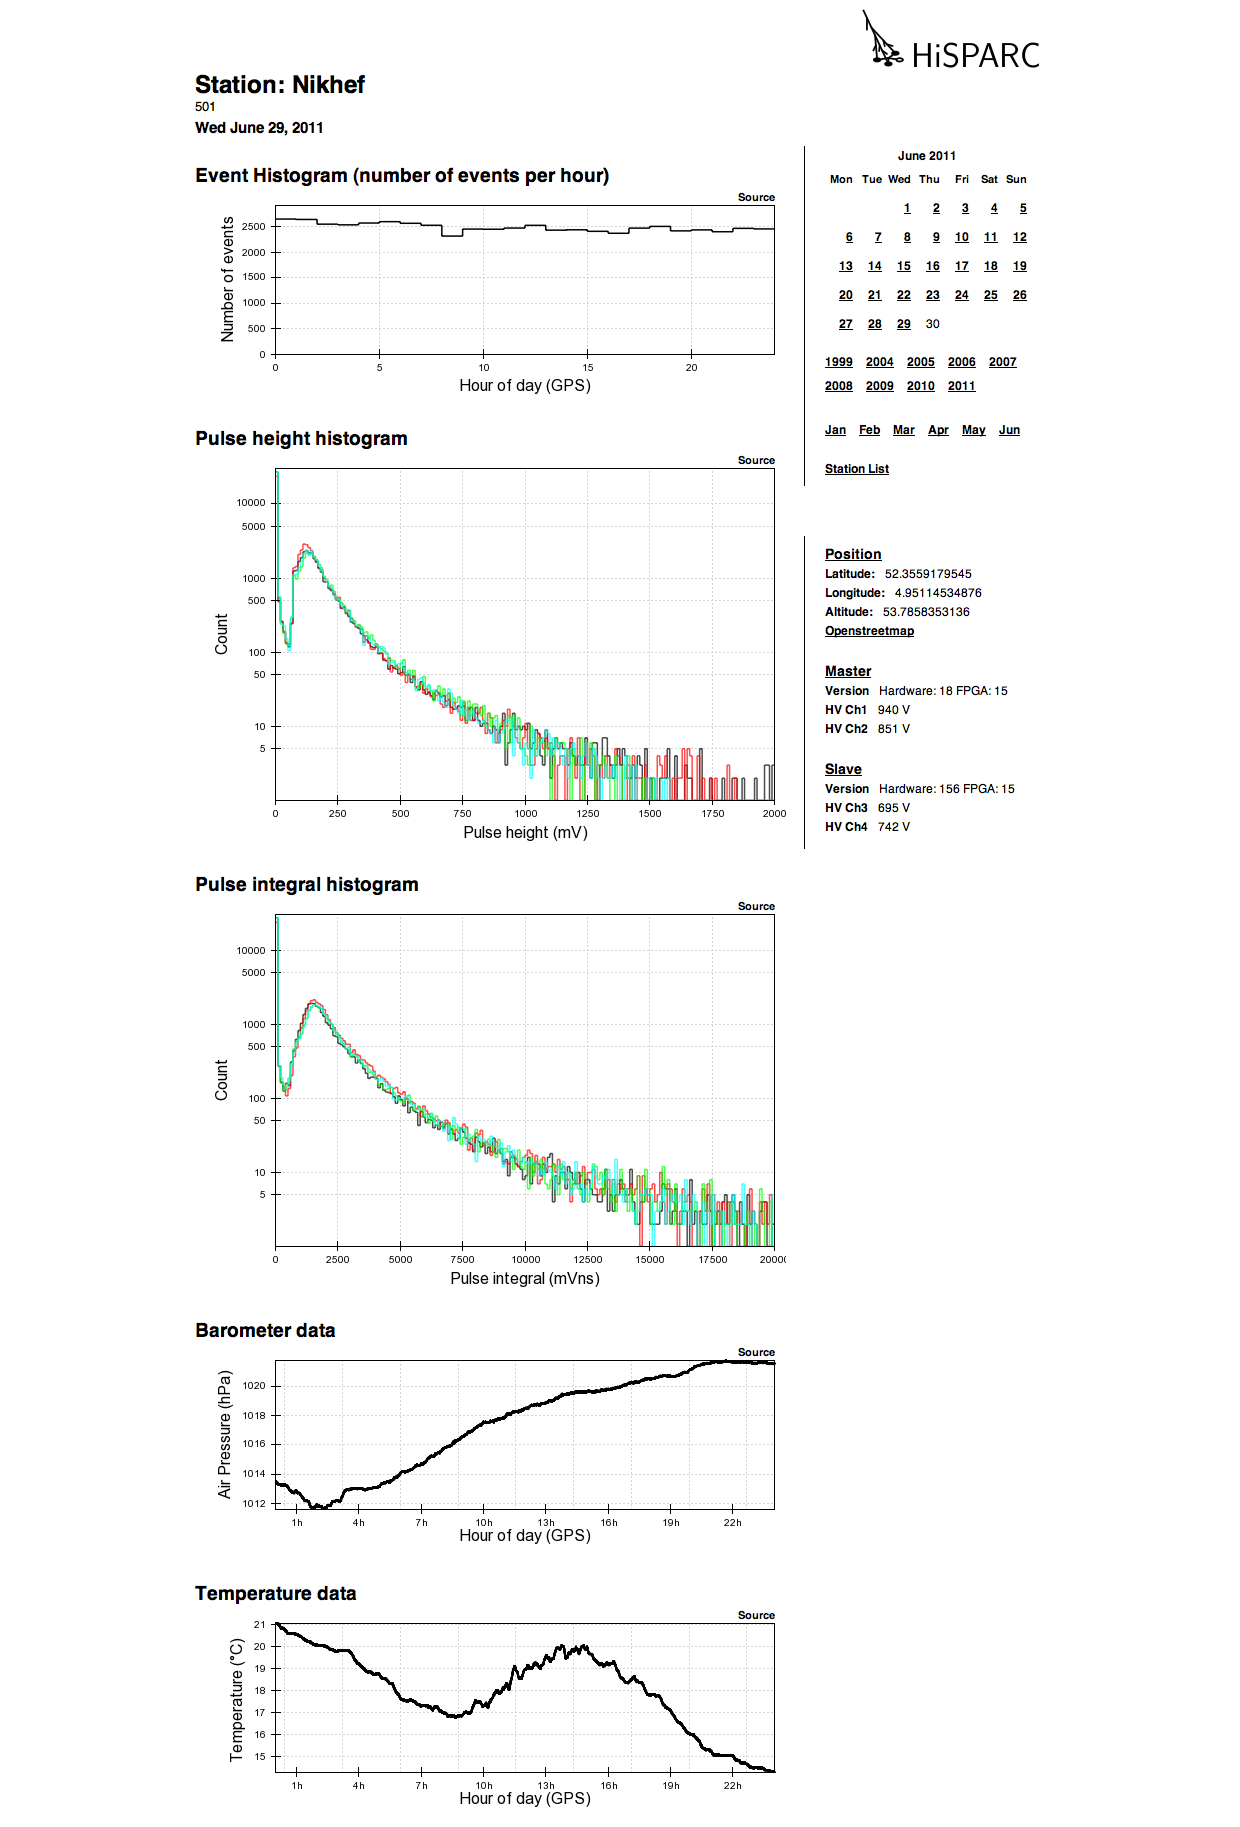
\includegraphics[height=.9\textheight]{figures/quicklooks-screenshot}
\caption{\captitle{Example of a quicklook page served by the public
database.}  This particular page can be found at
\url{http://data.hisparc.nl/django/show/stations/501/2011/6/29/}.}
\label{fig:quicklooks-screenshot}
\end{figure}

The quicklooks are, for example, useful for inspecting the quality of the data
for a given station (\figref{fig:quicklooks-screenshot}) or quickly observing
whether stations in the same area have seen an increase in event count during a
thunderstorm.  These pages also provide links to download the histogram data.

Each night, a cron job runs on the public database server to determine which
stations have received new data since the last time it was run.  Then, the event
data is read from the datastore using a read-only data connection and histograms
and datasets are generated for the quicklook pages.  This data is stored in a
MySQL database running on the public database server.  This database further
acts as the backend storage for the complete Django application.

Several analysis tools use the public database API to fetch events
and submit results.  Work is underway to make a few of them available at
\url{http://data.hisparc.nl/} to be used in a classroom setting.  The public
database API further defines the only public interface to accessing \hisparc
event data.  Since the public database itself only has a read-only connection to
the datastore, enforced by the OS of the datastore server, \emph{not} the OS of
the public database server, data integrity is assured.


\section{Monitoring and Control}

The \hisparc experiment is a large distributed network with stations being
maintained by high school teachers, support staff and students.  Since students
usually only work on \hisparc for a few months before graduating, and even
teachers move on to teaching other grades or at another location, \hisparc
stations need to run reliably without supervision for extended periods of time.
To make sure that they do, a system of monitoring is employed which ensures that
the \hisparc support team has access to information both offline (from
analyzing the data) and online (from the running station).  In case of problems,
accessing the station PC and making adjustments, or restarting the detector,
may become necessary.
This, too, is realized within this framework.

Each station receives an X.509v3 certificate which uniquely defines the station
PC, along with copies of the public certificates of the \emph{Virtual Private
Network (VPN)} server running OpenVPN \cite{OpenVPN}.  Each station contacts the
VPN server on start up and is connected to the \hisparc VPN network using strong
encryption. Strict firewall rules make sure that no data can be exchanged
between different station PCs.  A very restricted set of individuals also
receive special-purpose certificates and can connect to the \hisparc
\emph{administration VPN}, which is logically different from the station VPN
network.

There are only two types of connection allowed over the VPN:
\begin{enumerate}
    \item diagnostic data between a station PC and the VPN server
    \item remote desktop connections from an administrator PC to a station
    PC
\end{enumerate}
\figref{fig:vpn-connections} shows the connections which are allowed over the
VPN (dashed black lines) and the connections which are forbidden (dashed red
lines).
\begin{figure}
\centering
\begin{tikzpicture}[
    font=\sffamily,
    station/.style={draw,thick,rounded corners,fill=yellow!20,inner sep=.3cm},
    nagios/.style={draw,thick,rounded corners,fill=blue!20,inner sep=.3cm},
    admin/.style={draw,thick,rounded corners,fill=green!20,inner sep=.3cm},
    vpn/.style={draw,thick,fill=black!10},
    connect/.style={<->,>=stealth',shorten >=1pt,shorten <=1pt,semithick},
    forbidden/.style={red,dashed,semithick},
    decoration={markings,mark=at position .5 with {\draw[solid] (-3pt, -3pt) -- (3pt, 3pt); \draw[solid] (-3pt, 3pt) -- (3pt, -3pt);}},
    allowed/.style={dashed,semithick},
]
\pgfmathsetmacro{\radius}{1};
\pgfmathsetmacro{\labelradius}{3};

\draw[vpn] (0, 0) circle (\radius);
\node[right=1cm] (0, 0) {VPN server};

\coordinate (S1) at (150:\radius);
\node[station] (S1') at (150:\labelradius) {station};
\coordinate (S2) at (30:\radius);
\node[station] (S2') at (30:\labelradius) {station};
\coordinate (N) at (270:\radius);
\node[nagios] (N') at (270:\labelradius) {Nagios};
\coordinate (A) at (210:\radius);
\node[admin] (A') at (210:\labelradius) {administrator};

\draw[connect] (S1') -- (S1);
\draw[connect] (S2') -- (S2);
\draw[connect] (N') -- (N);
\draw[connect] (A') -- (A);

\draw[forbidden,postaction={decorate}] (S1) to[out=-30,in=210] (S2);
\draw[allowed] (S1) to[out=-30,in=90] (N);
\draw[allowed] (S2) to[out=210,in=90] (N);
\draw[allowed] (A) to[out=30,in=-30] (S1);

\end{tikzpicture}

\caption{\captitle{Allowed and forbidden VPN connections.}  Stations
and administrators connect to the VPN server using strong encrypted
connections.  The Nagios server connects to the VPN server on the local
network.  Strict firewall rules allow (black, dashed lines) or forbid (red,
dashed line) connections.  Connections between the Nagios server and the
stations are allowed, as well as connections from administrators to stations.
Connections between stations are strictly forbidden.}
\label{fig:vpn-connections}
\end{figure}

The VPN server runs an instance of the \emph{Nagios monitoring
system} \cite{Nagios} which can exchange diagnostic messages with the station
PCs.
\begin{figure}
\centering
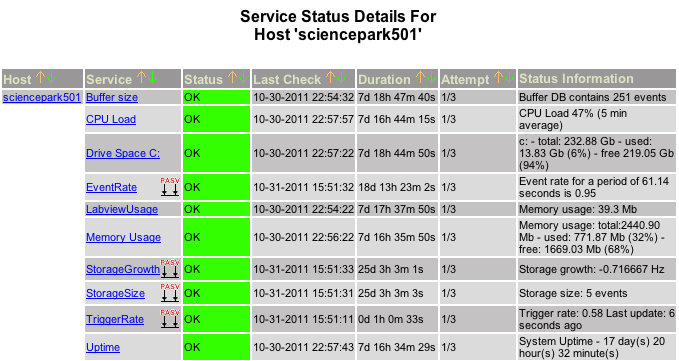
\includegraphics[width=\linewidth]{figures/screenshot-nagios}
\caption{\captitle{Screenshot of part of the Nagios user interface.}  This
screenshot shows the status of station 501 (Nikhef).}
\label{fig:nagios}
\end{figure}
Basic checks like uptime and disk and memory usage are performed, but
also more specific checks like the number of events residing in the Storage on
the station PC.  This information can be accessed using a web interface provided
by Nagios, and is a more rapid, albeit more basic, alternative to using the
data quicklooks to check on station health (\figref{fig:nagios}).

When an administrator wants to access a station PC to perform maintenance, he
connects to the administration VPN and can initiate a remote desktop connection
to any station PC.  The remote desktop software chosen for this purpose is
\emph{TightVNC} \cite{TightVNC}.  Its main advantage over other solutions,
like RDP\footnote{Remote Desktop Protocol (RDP) can be used to initiate a new session
on a remote Windows PC.}, is that it takes over the currently running session,
instead of creating a new session by way of login.  This way, remote assistance
can be provided and the software running on the current desktop can be accessed.


\section{Station Software}

The software running on the \hisparc station PC is installed by one installer
package.  This package not only installs software developed by \hisparc, but
also all third-party software packages which are in use.  The installer consists
of three components: the \emph{main installer}, the \emph{admin updater} and the
\emph{user updater}.

The main installer prepares the system for the station software and presents a
graphical user interface during installation.  Then, it unpacks the admin and
user updater packages and runs them one after another.  The admin updater
contains all the software which must be installed and run using administrator
rights.  This includes:
\begin{description}
\item[niruntime]  The National Instruments \labview runtime engine.  This is
needed to run the \daq programs.
\item[openvpn]  The virtual private network, running as a service.
\item[tightvnc] The remote desktop, running as a service.
\item[nsclient++] The Nagios client, providing check results to the Nagios
server, running as a service.
\item[drivers] Various drivers necessary for communication with the hardware,
and providing a connection from \labview to MySQL.
\end{description}
%
The user updater can be installed and run without administrator rights.  It is
thus possible to distribute user updates and have the software installed by
regular users, or by software running without administrator rights.  The user
updater includes:
\begin{description}
\item[diagnostictool]  A troubleshooting tool for performing diagnostic checks.
\item[dspmon]  A program used to read out and program the GPS receiver in the
\hisparc electronics unit.
\item[hisparcdaq]  The \hisparc \daq software.
\item[hisparcweather]  The weather station \daq software
\item[hsmonitor]  The \hisparc monitor application, collecting and uploading
\hisparc and weather station data.  It also provides periodic check results to
Nagios.
\item[mysql]  The MySQL server
\item[python]  The Python interpreter and standard libraries
\item[updater]  The updater program, which periodically checks for software
updates.
\end{description}
%
The updater downloads software updates.  If an admin update is available, the
user is notified to log in as an administrator to run the update.  If a user
update is available, all user software is shut down, the update is performed,
and the software is restarted.  This mechanism proved necessary to make sure
that all station PCs are running up-to-date software.


\section{SAPPHiRE}

The results of many experiments are compared to simulations of the physics
behind the experiment.  Often, simulations guide the design of the experiment.
The final results are documented in \emph{Technical Design Reports}, e.g.
\cite[29]{Atlas:TDR}. The bulk of the simulation code is usually shared between
scientists, with different implementations of, and additions to, various parts
of the code.  The same holds true for the analysis of experimental results.

Generally, the problem of managing the code is solved by creating a
\emph{framework}.  A framework enables researchers to use the exact same code,
while being able to extend the code with additions and reimplementations of
various parts.  If useful, these contributions can then be added to the
framework, to the benefit of all users.


\subsection{Frameworks}

A framework is different from a software \emph{library}, which is a collection
of functions that can be used in programs to perform various tasks.  However, a
framework can \emph{evolve} from a library.  The differences can be summarized
as follows \cite{Fayad:1997}:
\begin{enumerate}
    \item modularity
    \item reusability
    \item extensibility
    \item inversion of control
\end{enumerate}
%
The \emph{modularity} of a framework ensures that key concepts and
implementations of a certain aspect of the functionality is kept together, in
one part of the framework.  This can be accomplished by designing classes with
limited functionality which do not depend on implementation details of other
classes.  Furthermore, classes can be grouped together depending on their
function and a hierarchy can be defined by using \emph{namespaces}.  For
example, a \verb|simulations.detector.ScintillatorSimulation| class does not
depend on the implementation details of
\verb|simulations.detector.PMTSimulation|, but may share a common interface.
Such common interfaces promote \emph{reusability}, where components of the
framework can be easily reused in user applications.  If a framework is highly
modular, reusing a class has no side-effects.  For example, a user can be
ensured that using a \verb|DirectionReconstruction| class does not require a
simulation to be performed first.  Common interfaces result in the possibility
of exchanging a \verb|FullDetectorSimulation| with a
\verb|ToyMonteCarloDetectorSimulation| by changing only one line of code.

\emph{Extensibility} is a necessary feature of a framework.  Scientists need to
override parts of the framework, like simulation algorithms, with custom
versions to investigate their behavior.  The framework ensures that common code
is shared, while custom code can be incorporated.  It is important to note that
this custom code is not defined \emph{in the framework}, but is defined only in
the user application.  If useful, new algorithms can be submitted and
incorporated in the framework itself for use by other users.

Another important aspect of frameworks is \emph{inversion of control}.  In
applications using libraries the control flow of a program is defined by the
application code.  The code calls functions and methods of the library when it
sees fit.  Complex tasks which are handled by the library can't be extended by
the program.  Frameworks allow users to extend and alter the framework.  The
framework contains a skeleton of a complex flow, e.g. an analysis procedure, and
allow user programs to supply classes which handle certain tasks.  The flow of
control is handled by the framework, not the program.  The program does not call
methods of the framework one after another to complete a task.  Rather, the
framework calls parts of the user program to perform aspects of the task at
hand.  The flow is under control of the framework, and thus the control is
\emph{inverted}.

Modularity, reusability, extensibility and inversion of control are closely
related and each of them enables the others.


\subsection{The HiSPARC Framework}

Reusing common parts of simulation and analysis programs can result in a library
shared by a group of scientists.  This library can be both modular and reusable.
Only when program \emph{flow} needs to be shared in an extensible way, a
framework can result as an evolution of the library.  This is contrary to the
situation in which a framework is designed up-front by first specifying all
requirements and then implementing them.  It is common for a framework to be the
result of both.

The code used by the \hisparc experiment started life as a library of functions
for downloading data and processing events.  Early simulations were added as
functions as well.  While the library had multiple, modular, components, it was
not easily extensible.  The requirement of more complex analysis procedures
which needed to work on both simulated and experimental data resulted in common
interfaces and inversion of control.  Finally, extensibility was incorporated
into the design.  The resulting framework was clearly an evolution of the
library, with some later parts designed up-front.

\sapphire stands for Simulation and Analysis Program Package for \hisparc
Research and Education.  It's purpose is to be used heavily by researchers
performing simulation and analysis tasks, as well as high school and university
students who need easy access to the data and analysis tools.  Light reflections
in blue sapphires are reminiscent of the blue / violet color of scintillation
light in the common scintillator used by \hisparc.

As the name suggests, the two main components of the framework are simulation
and analysis.  The simulation component includes classes to perform event
simulation based on the results from full Monte Carlo EAS simulations, or
lateral distribution functions.  Also, these simulations can be performed
running on a local workstation or a cluster like the Nikhef Stoomboot cluster, just by
switching classes in one line of code.  An example of code using \sapphire is
shown in \figref{fig:sapphire-example}.  An event simulation of the Science Park
Array is run by simulating \num{1000000} showers, making use of a lateral
distribution function derived from analysis of data in the \kascade experiment.
For each simulated event the core position is reconstructed using a new
algorithm defined in the user code.  This algorithm is a subclass of the
framework-supplied algorithm and possibly overrides only a small part of the
algorithm.  Storage of the reconstruction results is still fully handled by the
framework and thus compatible with all existing visualization tools.

\begin{figure}
\begin{minted}{python}
import tables

from sapphire.clusters import SciencePark
from sapphire.simulations.ldf import KascadeLdfSimulation
from sapphire.analysis.core_reconstruction import CoreReconstruction, \
                                                  CorePositionSolver


class MyCorePositionSolver(CorePositionSolver):
    """Implements some new algorithm"""
    #...
    pass


def plot_reconstruction_results(results_table):
    """Generates a set of plots for review"""
    #...
    pass


if __name__ == '__main__':
    data = tables.openFile('my_data.h5', 'w')

    # simulation
    cluster = SciencePark()
    simulation_results = '/simulations/ldf/run_1'
    sim = KascadeLdfSimulation(data, cluster, simulation_results, N=1e6)
    sim.run()

    # reconstruction
    reconstruction_results = '/reconstructions/ldf'
    rec = CoreReconstruction(data, reconstruction_results)
    rec.reconstruct_core_positions(simulation_results,
                                   solver=MyCorePositionSolver())

    plot_reconstruction_results(data, reconstruction_results)
\end{minted}
\caption{\captitle{SAPPHiRE example code.}  This code performs a simulation
using lateral distribution functions of \num{1000000} showers and reconstructs
core positions using a user-supplied algorithm.  Storing simulation and
reconstruction results inside a group hierarchy is fully handled by the
framework.  This code makes use of default values of the framework, e.g.
the shower size.}
\label{fig:sapphire-example}
\end{figure}

\sapphire will be extensively documented in \cite{SAPPHiRE}.


\section{Software Management}

Software development practices can be grouped in various schools of thought
which sometimes are at odds with each other.  For example, the \emph{waterfall
model} \cite{Royce:1970} defines a sequential design process.  This process is
defined in the following order: requirements, design, implementation,
verification and maintenance.  The requirements and design of the software are
completed before work is started on the implementation.  On the other
hand, \emph{agile software development} \cites{agile}{agile-manifesto} advocates
processes and methods based on iterative and incremental development, resulting
in an evolution of requirements and solutions.

The one thing that all schools of thought agree on is the need for
\emph{revision control}, or \emph{version control}.  The software changes
substantially during development and it usually becomes necessary at some point
to know exactly which changes were introduced during a certain development
phase.  Possible reasons include uncovering bugs which were introduced after a
certain date.  Ad hoc solutions like copying code to directories with versioned
names like \verb|code-2008-02-19| are very fragile.  Especially when working in
teams, merging code changes from various members can introduce subtle side
effects.

Revision control systems solve the problem of managing an evolving code base by
storing many versions of the code in one location, called a \emph{repository},
and providing various tools to explore the differences between versions and
reverting parts of the code to earlier versions.  Over the years, many such
systems were created.  At first, such systems stored all the code and history in
one central location, and are thus called \emph{centralized}.  Popular systems
include \emph{CVS} and \emph{Subversion}.  More recently, \emph{distributed}
systems were created, like \emph{Bazaar, Mercurial} and \emph{Git}.  Distributed
systems store all the history and code locally and each users repository is on
equal footing.  Usually a distributed workflow is combined with a central
location containing the copy used to created software releases.  This copy is
updated by all team members when new features are implemented.

Revision control systems often include tools to create \emph{branches} of the
code, in which a certain feature can be developed independently of changes to
the \emph{master}, or \emph{trunk}, branch.  When such a feature is ready for
inclusion, it is \emph{merged} back into the master branch.  Systems like Git
encourage heavy use of branching and include powerful tools for merging the
changes.  Distributed systems are more compatible with agile development methods
in that they evolve along with the changing work flow of software projects.  For
example, there is no need to set up a central repository.  A single developer
issues a \verb|git init| inside his project directory and starts developing and
\emph{committing} changes to the repository.  This repository can then be shared
with other developers when the need arises and changes can flow both ways.  If
the team grows, it may become preferable to create a central location which is
kept in sync with all developers' copies.

The \hisparc project has used revision control since 2008.  At first, Bazaar
\cite{Bazaar} was used because of its excellent documentation.  Recently, all
repositories were converted to use Git \cite{Git} and the repositories are now
hosted on Github \cite{github}.  Github simplifies the hosting of code and
includes an \emph{issue tracker}, which allows anyone to report a bug.
The problem and possible solutions can then be discussed in one central
location.  Git (and Github) give all team members a powerful work flow by easily
visualizing changes, develop new features or fix bugs in isolation, and merge
the changes into the master branch.  By making development public,
accountability is increased, which promotes the use of \emph{clean code}.
Furthermore, any user can \emph{fork}\footnote{Essentially making a copy of the
repository to start development independently of the parent repository.} the
repository and fix bugs or add features.  They can then issue a \emph{pull
request}, which asks the team developing the main repository to include the
changes.  Bachelor or Master students can thus immediately use and alter the
\hisparc software, without giving them any rights to the main repositories.

The home page for \hisparc on Github is located at
\url{http://github.com/HiSPARC/}.  It includes the following repositories:
\begin{description}
\item[datastore]  The code running the central datastore.  It is responsible for
first accepting the data and for aggregating the data and storing it in binary
\hdf files.
\item[labview]  The code for the \hisparc \daq software.
\item[publicdb]  The code for the public database, which is a Django application
running at \url{http://data.hisparc.nl/}.
\item[sapphire]  The code of the \sapphire framework, used for analyzing
\hisparc data and simulating events.
\item[station-software] The code running on station PCs, including the code for
building the installer package, with the exception of \labview sources.  The
\hisparc \daq software, as well as the weather station \daq software, have their
own repositories.  All other code, including third-party components, is located
in this repository.  The most important piece of code in this package is the
\emph{monitor}, responsible for uploading data and sending check results to the
Nagios instance running on \url{http://vpn.hisparc.nl/}.
\item[vhdl]  The source of the \textsmaller{VHDL} code used to program the
\textsmaller{FPGA} unit inside the \hisparc electronics module.
\item[weather]  The code for the weather station \daq software.
\end{description}
%
All repositories have their own issue tracker and most contain documentation
describing the code base and instructions on how to set up a development
environment.  Access rights can be specified by including developers into
\emph{teams}, which can be assigned to one or multiple repositories.  Each
repository can grant write access to multiple teams.  Development is completely
open, however, and everyone has read access.

Using Github, the \hisparc experiment has extended its outreach character to
include not only cosmic ray research, but also all aspects of software
development.
